\subsection{Lead vs Aluminium}
\label{Lead vs Aluminium SubSection}

Lead is a dense metal, which is why certain types of radiation cannot penetrate fully through, its also why lead makes for a good material to use for radiation shielding. An experiment \cite{GammaRay} to measure gamma ray particle counts through lead and aluminium over time was conducted, where a decaying radioactive isotope Cesium 137 is suspended above various thicknesses or lead and aluminium to measure the particle count able to penetrate through the two materials. In \cref{Data1} and \cref{Data 2} shows the count for lead and aluminium respectfully where the experiment proved that the gamma ray particle count when the thickness of the lead material is increased lowers due to the highly dense material blocking/ absorbing the particles. Whereas with the material aluminium in \cref{Data 2} shows minimal change of the particle count as the material thickness increases do to aluminium being less dense. The density of both materials is seen through their independent physical properties; lead is heavy and less malleable whereas aluminium is light and highly malleable. 

\newpage
\begin{figure}[H]
\centering
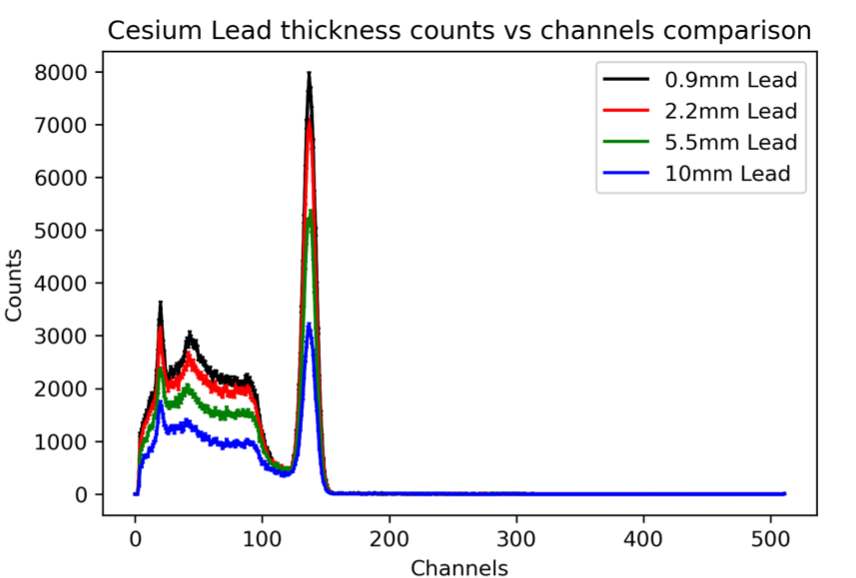
\includegraphics[scale=0.9]{Media/DataAnalysis/Screenshot 2021-03-15 at 05.49.36.png}
\caption{Graphical representation of energy counts vs time from Cesium 137 through various Lead thicknesses \cite{GammaRay}}
\label{Data 1}
\end{figure}

\begin{figure}[H]
\centering
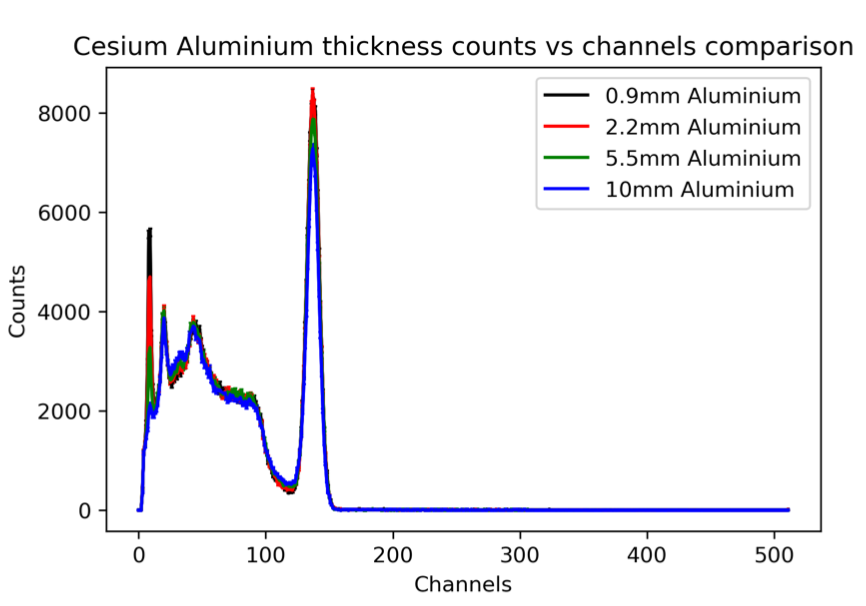
\includegraphics[scale=0.9]{Media/DataAnalysis/Screenshot 2021-03-15 at 05.49.54.png}
\caption{Graphical representation of energy counts vs time from Cesium 137 through various Aluminium thicknesses \cite{GammaRay}}
\label{Data 2}
\end{figure}